\documentclass[border=6pt]{standalone}
\usepackage{tikz}
\usepackage{amsmath}
\usetikzlibrary{arrows.meta,positioning,fit,backgrounds,calc}
\definecolor{cBench}{HTML}{2E6E8E}
\definecolor{cBenchBg}{HTML}{E4EFF4}
\definecolor{cLoop}{HTML}{1A9E8F}
\definecolor{cLoopBg}{HTML}{E1F3EF}
\definecolor{cTester}{HTML}{C1440E}
\definecolor{cTesterBg}{HTML}{FBEBE1}
\definecolor{cEval}{HTML}{9C3B7A}
\definecolor{cEvalBg}{HTML}{F4E7F0}
\definecolor{cInk}{HTML}{222222}
\begin{document}
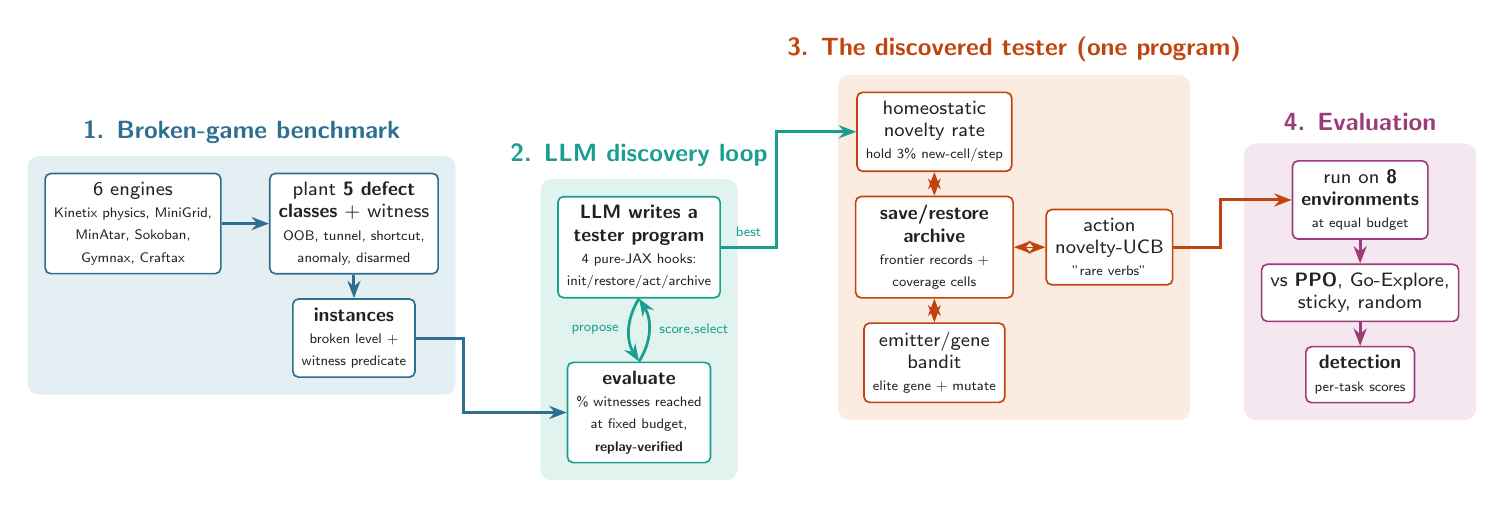
\begin{tikzpicture}[
  font=\sffamily,
  >={Stealth[length=2.2mm]},
  mod/.style={rounded corners=2pt, draw=#1, fill=white, line width=0.6pt, inner sep=3.2pt, align=center, text=cInk, font=\sffamily\scriptsize, minimum height=7mm},
  stagelbl/.style={font=\sffamily\bfseries\small, text=#1},
  flow/.style={->, line width=1.1pt, draw=#1},
  loop/.style={->, line width=1.0pt, draw=cLoop},
]

% ===================== Stage 1: benchmark =====================
\node[mod=cBench] (engines) {6 engines\\{\tiny Kinetix physics, MiniGrid,}\\{\tiny MinAtar, Sokoban,}\\{\tiny Gymnax, Craftax}};
\node[mod=cBench, right=6mm of engines] (inject) {plant \textbf{5 defect}\\\textbf{classes} + witness\\{\tiny OOB, tunnel, shortcut,}\\{\tiny anomaly, disarmed}};
\node[mod=cBench, below=3mm of inject] (inst) {\textbf{instances}\\{\tiny broken level +}\\{\tiny witness predicate}};
\draw[flow=cBench] (engines) -- (inject);
\draw[flow=cBench] (inject) -- (inst);

% ===================== Stage 2: LLM discovery loop =====================
\node[mod=cLoop, right=15mm of inject, yshift=-3mm] (llm) {\textbf{LLM writes a}\\\textbf{tester program}\\{\tiny 4 pure-JAX hooks:}\\{\tiny init/restore/act/archive}};
\node[mod=cLoop, below=8mm of llm] (fit) {\textbf{evaluate}\\{\tiny \% witnesses reached}\\{\tiny at fixed budget,}\\{\tiny \textbf{replay-verified}}};
\draw[loop] (llm.south) to[bend right=32] node[left, font=\sffamily\tiny, text=cLoop] {propose} (fit.north);
\draw[loop] (fit.north) to[bend right=32] node[right, font=\sffamily\tiny, text=cLoop] {score,\\select} (llm.south);
\draw[flow=cBench] (inst.east) -- ($(inst.east)+(6mm,0)$) |- (fit.west);

% ===================== Stage 3: the discovered tester =====================
\node[mod=cTester, right=17mm of llm, minimum width=20mm] (arch) {\textbf{save/restore}\\\textbf{archive}\\{\tiny frontier records +}\\{\tiny coverage cells}};
\node[mod=cTester, above=3mm of arch] (homeo) {homeostatic\\novelty rate\\{\tiny hold 3\% new-cell/step}};
\node[mod=cTester, below=3mm of arch] (bandit) {emitter/gene\\bandit\\{\tiny elite gene + mutate}};
\node[mod=cTester, right=4mm of arch] (ucb) {action\\novelty-UCB\\{\tiny "rare verbs"}};
\draw[flow=cLoop] (llm.east) -- node[above, font=\sffamily\tiny, text=cLoop]{best} ($(llm.east)+(7mm,0)$) |- (homeo.west);
\draw[<->, line width=0.5pt, draw=cTester] (homeo) -- (arch);
\draw[<->, line width=0.5pt, draw=cTester] (bandit) -- (arch);
\draw[<->, line width=0.5pt, draw=cTester] (arch) -- (ucb);

% ===================== Stage 4: evaluation =====================
\node[mod=cEval, right=15mm of ucb, yshift=6mm] (run) {run on \textbf{8}\\\textbf{environments}\\{\tiny at equal budget}};
\node[mod=cEval, below=3mm of run] (vs) {vs \textbf{PPO}, Go-Explore,\\sticky, random};
\node[mod=cEval, below=3mm of vs] (out) {\textbf{detection}\\{\tiny per-task scores}};
\draw[flow=cTester] (ucb.east) -- ($(ucb.east)+(6mm,0)$) |- (run.west);
\draw[flow=cEval] (run) -- (vs);
\draw[flow=cEval] (vs) -- (out);

% ===================== stage backdrops + titles =====================
\begin{scope}[on background layer]
  \node[fill=cBenchBg, rounded corners=4pt, fit=(engines)(inject)(inst), inner sep=6pt] (b1) {};
  \node[fill=cLoopBg, rounded corners=4pt, fit=(llm)(fit), inner sep=6pt] (b2) {};
  \node[fill=cTesterBg, rounded corners=4pt, fit=(homeo)(arch)(bandit)(ucb), inner sep=6pt] (b3) {};
  \node[fill=cEvalBg, rounded corners=4pt, fit=(run)(vs)(out), inner sep=6pt] (b4) {};
\end{scope}
\node[stagelbl=cBench, above=1pt of b1.north] {1. Broken-game benchmark};
\node[stagelbl=cLoop, above=1pt of b2.north] {2. LLM discovery loop};
\node[stagelbl=cTester, above=1pt of b3.north] {3. The discovered tester (one program)};
\node[stagelbl=cEval, above=1pt of b4.north] {4. Evaluation};
\end{tikzpicture}
\end{document}
